\section{Gestione del Database}

\subsection{Diagramma E-R}
Il diagramma entità-relazione (progetto concettuale) è formato dalle entità che entrano in gioco in SWIMv2 e dalle relazioni che intercorrono tra di esse; è un passo intermedio
verso la definizione delle tabelle del database del sistema e mette in evidenza in che modo le entità interagiscono tra di loro.
\\[2\baselineskip]
\noindent
Il diagramma è questo (segue spiegazione delle entità e delle relazioni):
\vspace{1cm}
\begin{center}
 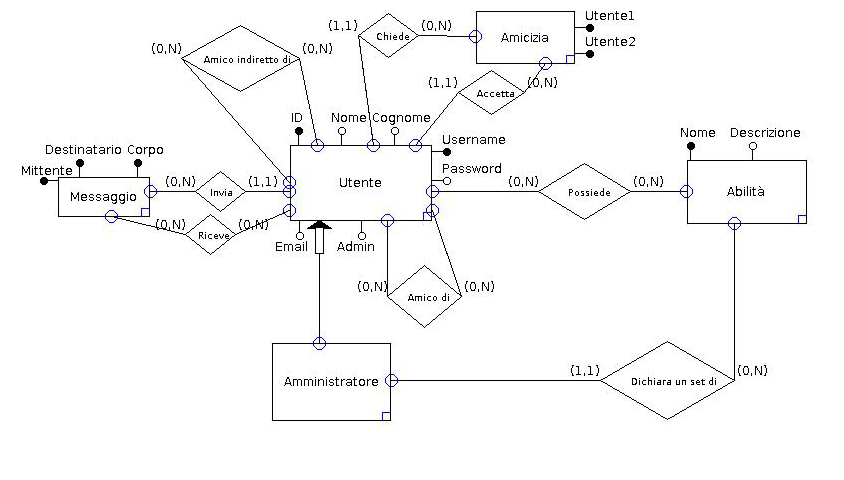
\includegraphics[width=1.1\columnwidth]{ER.png}
\end{center}

\subsubsection{Entit\'a}
\begin{itemize}
 \item {\bfseries Utente}: è l'entità principale e contiente i dati della persona che si è registrata su SWIMv2: nome, cognome, indirizzo email, username e password, oltre ad un campo
 univoco ID e ad un campo Admin (che nella tabella sarà di tipo tinyint(1)) che indica se l'utente è o non è un amministratore.
 \item {\bfseries Amministratore}: è un sottotipo di utente che ha delle funzionalità in più: può infatti gestire il set di abilità di sistema.
 \item {\bfseries Messaggio}: è un entità che modella i messaggi tra gli utenti: infatti ha come attributi il mittente, il destinatario e il corpo.
 \item {\bfseries Abilità}: è un entità che indica il set di abilità di sistema da cui gli utenti possono dichiarare le proprie abilità.
 \item {\bfseries Amicizia}: indice il fatto che due utenti siano amici tra di loro, e infatti i suoi attributi sono proprio tali utenti
\end{itemize}

\subsubsection{Relazioni}
\begin{itemize}
 \item {\bfseries Chiede - Accetta}: sono riferite al fatto che un utente possa chiedere o accettare una richiesta di amicizia a/da un altro utente.
 \item {\bfseries Invia - Riceve}: sono riferite al fatto che un utente possa inviare o ricevere un messaggio
 \item {\bfseries Amico diretto - Amico indiretto}: sono riferite al fatto che un utente possa essere amico diretto o indiretto di un altro amico
 \item {\bfseries Possiede}: è riferita al fatto che ogni utente possiede un set di abilità
 \item {\bfseries Utente}: è riferita al fatto che un amministratore può modificare il set di abilità di sistema
\end{itemize}

\subsection{Progetto Logico}
Il progetto logico consiste nell'insieme di tabelle che compongono il database, ottenute a partire dall'ER.
\subsubsection{Tabelle risultanti}
\noindent
UTENTE({\bfseries ID},NOME,COGNOME,EMAIL,{\bfseries USERNAME},PASSWORD,ADMIN)\\
ABILITA'({\bfseries NOME},DESCRIZIONE)\\
ABILITA'UTENTI({\bfseries UTENTE,ABILITA'})\\
MESSAGGIO({\bfseries ID,MITTENTE,DESTINATARIO},CORPO)\\
AMICIZIA({\bfseries UTENTE1,UTENTE2})\\
FEEDBACK({\bfseries ID, UTENTE1, UTENTE2}, VOTO)\\

\noindent
in cui in ABILITA'UTENTI.NOME si riferisce a UTENTE.USERNAME, ABILITA'UTENTI.ABILITA' si riferisce a ABILITA'.NOME, MESSAGGIO.MITTENTE, MESSAGGIO.DESTINATARIO, AMICIZIA.UTENTE1,
AMICIZIA.UTENTE2, FEEDBACK.UTENTE1 e FEEDBACK.UTENTE2 si riferiscono tutti a UTENTE.USERNAME. Le chiavi primarie sono in grassetto.

\subsection{Vista Logica}
L'ultimo diagramma relativo al database è la vista logica delle tabelle del database:
\begin{center}
 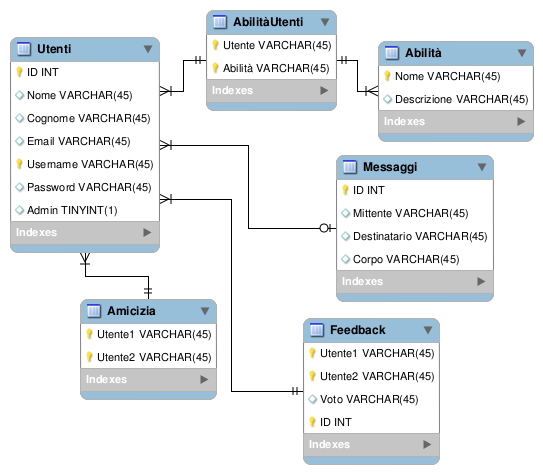
\includegraphics[width=1\columnwidth]{logico.png}
\end{center}